\section{Voltage Reference}

\begin{figure}[H]
\centering
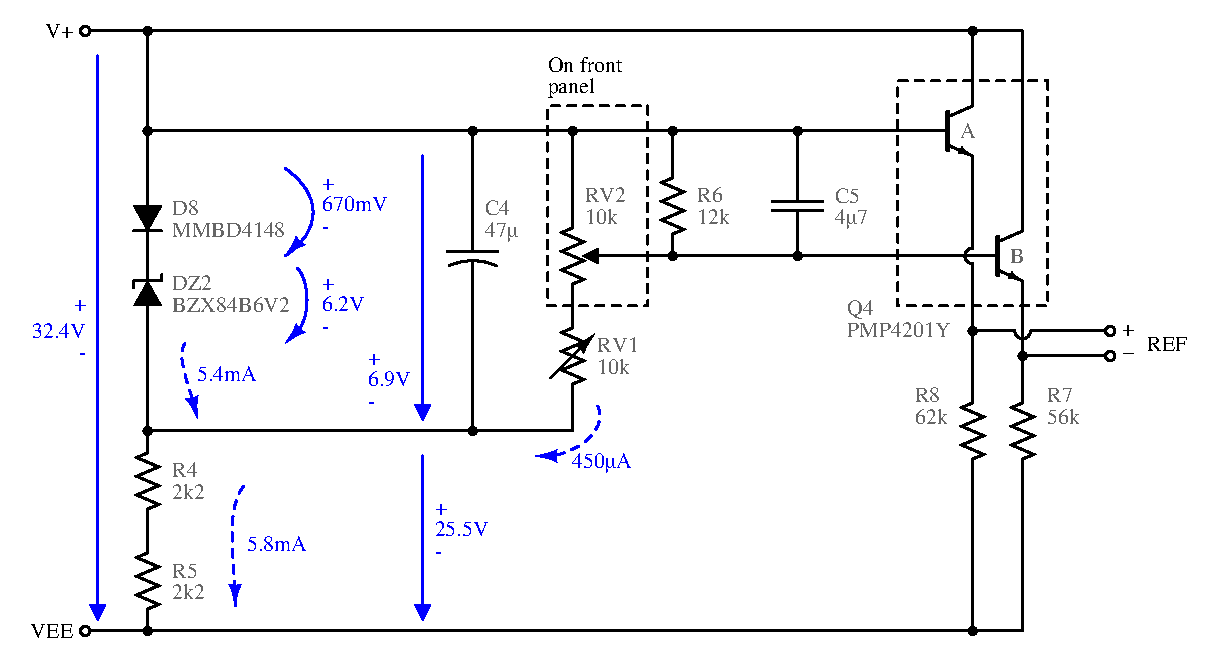
\includegraphics[width=5.5in]{sch/reference}
\caption{Voltage reference sub-schematic}
\label{fig:reference}
\end{figure}

\begin{multicols}{2}
To allow the power supply to output a fixed voltage, a voltage reference
circuit is used. This is essentially a second regulator, and because it is
run from the main regulator, the input power rejection compounds with that
of the main regulator.

\subsubsection{Reference Diode}
Zener diode \texttt{DZ2}, another BZX84-series 2~\% reference diode, is combined
with a standard MMBD4148 (surface-mount equivalent to the well known 1N4148)
in a sort of compound diode. The reason for this is temperature coefficients:
\end{multicols}

\begin{table}[H]
\centering
\begin{tabular}{l|llll}
 & & \multicolumn{3}{c}{Temperature error, mV/\dg C} \\
Diode & Voltage at 5~mA bias & (min) & (typ) & (max) \\
\hline
MMBD4148 & 670~mV & & -2 & \\
BZX84B6V2 & 6.2~V & 0.4 & 2.3 & 2.7 \\
\hline
Total & 6.87~V & -1.6 & 0.3 & 0.7 \\
\end{tabular}
\end{table}


\begin{multicols}{2}
Note that temperature coefficient of standard silicon PN diodes like the 4148
is much more regular, so only a `typical' value was given. This combination
gives a compound diode with a typical variation of only 0.3~mV/\dg C, or
0.09~\% over the full temperature range.

\subsubsection{Biasing}
Because only a pair of resistors (a pair, rather than just one, to share heat,
as they will get warm) is being used to supply current, there will be another
contribution to the error from the variation in VEE, calculated above. VEE can
have a drift-related (non-trimmable) error of up to 1.63~\%. This translates to
a variation in current through \texttt{R4} and \texttt{R5} of
$(0.0163)(32.4\;V-6.9\;V)/(4.4\;k\Omega) = 94.5\;\mu A$ in
either direction. The dynamic impedance of the BZX84B6V2, listed in the
datasheet, is no more than 10~$\Omega$. The dynamic impedance of the MMBD4148
is about 20~$\Omega$, which is not listed and must be measured from the
``Forward Voltage vs. Forward Current'' plot. This gives an error of up to
$(94.5\;\mu A)(30\;\Omega) = 2.84\;mV$ total, or 0.04~\%. Assuming the two
errors are not large enough to meaningfully affect each other, the total
non-trimmable error of the primary
reference is 0.13~\%.

\subsubsection{Potentiometer}
This reference voltage goes into front panel potentiometer \texttt{RV2}, and
a section of the voltage is trimmed off by \texttt{RV1} to compensate for
aforementioned variations in parts. \texttt{R6} ensures that if \texttt{RV2}'s
wiper becomes disconnected (a somewhat common failure mode in panel-type
potentiometers), the output voltage defaults to zero. \texttt{C5} provides
extra filtering to remove any noise picked up by the cable running to the
panel.

\subsubsection{Output Buffer}
\texttt{Q4} is a pair of NPN transistors, factory-selected to have nearly
identical
characteristics and mounted in one small package to ensure equal temperature.
Each transistor is used to buffer one side of the reference voltage, and
despite the approximately 650~mV drop, the relative voltage should still be
equal because of the matched characteristics. Buffering is necessary because
the error amplifier requires a known impedance of the input signals, but the
impedance at the output of a potentiometer changes drastically over the
range. The output impedance of an emitter follower is very low, and will be
dominated by the resistors in the error amplifier.

\texttt{R7} and \texttt{R8} are selected to give as close to equal currents
through each half of \texttt{Q4} as possible, without using an active current
source circuit. Using V+ as a reference ground for calculation, \texttt{Q4A}
will always see 0~V on its base, and so its emitter will give -0.65~V.
With VEE as -32.4~V, \texttt{R8} will see 31.75~V, drawing 512~$\mu$A.
As the potentiometer is turned, the voltage at \texttt{Q4B}'s base and emitter
will change, ranging from -0.65~V at the emitter to -5.30~V. This gives a
current range through \texttt{R7} from 484~$\mu$A to 567~$\mu$A, centered
at  525~$\mu$A.

\end{multicols}
